\textbf{Ejemplo 7}\\
Una industria puede adquirir una máquina a un costo de 6.000.000 COP, tendrá una vida útil de 5 años y prácticamente no tendrá valor de salvamento, la máquina será totalmente depreciada en 3 años por partes iguales, el estudio de mercados indica que los ingresos del primer año serán aproximadamente de 3.000.000 COP y aumentarán todos los años un 30\% periodo año vencido, por otra parte, se estima que el costo de producción del primer año será de 800.000 COP y cada año aumentará en 200.000 COP. Suponiendo una tasa impositiva del 38\% nominal anual año vencido. Determinar la rentabilidad del proyecto usando un horizonte de planeación de 5 años.
\\
\newpage
\textbf{Solución.}\\
%La tabla ira centrada
\begin{center}
	\renewcommand{\arraystretch}{1.5}% Margenes de las celdas
	%Creación de la cuadricula de 3 columnas
	\begin{longtable}[H]{|c|c|c|}
		%Creamos una linea horizontal
		\hline
		%Definimos el color de la primera fila
		\rowcolor[HTML]{FFB183}
		%%%%% INICIO ASIGNACIÓN PERÍODO FOCAL %%%%%%%
		%%%%%%%%%% INICIO TITULO
		%Lo que se hace aquí es mezclar las 3 columnas en una sola
		\multicolumn{3}{|c|}{\cellcolor[HTML]{FFB183}\textbf{1. Asignación período focal}}                                                                                                                                                                                             \\ \hline
		%%%%%%%%%% FIN TITULO
		%%%%% INICIO DECLARACIÓN DE VARIABLES %%%%%%%
		\multicolumn{3}{|c|}{$pf : 0pav$}                                                                                                                                                                                                                                              \\ \hline

		%%%%%%%%%%% INICIO TITULO
		\rowcolor[HTML]{FFB183}
		\multicolumn{3}{|c|}{\cellcolor[HTML]{FFB183}\textbf{2. Declaración de variables}}                                                                                                                                                                                             \\ \hline
		\multicolumn{1}{|c|}{\cellcolor[HTML]{FFB183}\phantom{000}\textbf{Valores monetarios}\phantom{000}} & \multicolumn{1}{c|}{\cellcolor[HTML]{FFB183}\phantom{000}\textbf{Valores no monetarios}\phantom{000}} & \multicolumn{1}{c|}{\cellcolor[HTML]{FFB183}\textbf{Incógnitas}} \\ \hline
		%%%%%%%%%%% FIN TITULO
		%%%%%%%%%%% INICIO MATEMÁTICAS
		$ P_{1} = 6\text{.}000\text{.}000 \text{ COP}$                                                      & $i_{1} = 30\% pav$                                                                                    & $ FNC = ? $                                                      \\
		$\textbf{Ingresos primer año}: 3\text{.}000\text{.}000\text{ COP}$                                  & $\textbf{Tasa impositiva}: i = 38\% pav$                                                              & $VPN = ?\text{ COP}$                                             \\
		$\textbf{Costo primer año}: 800\text{.}000\text{ COP}$                                              & $n = 5 pav$                                                                                           & $i_{R} = ? pav$                                                  \\
		$\textbf{Aumento coste por año}: 200\text{.}000\text{ COP}$                                         &                                                                                                       &                                                                  \\
		\hline
		%%%INICIO DIAGRAMA DE FLUJO
		%%INICIO TITULO
		\multicolumn{3}{|c|}{\cellcolor[HTML]{FFB183}\textbf{3. Diagrama de flujo de caja}}                                                                                                                                                                                            \\ \hline
		%%FIN TITULO
		%%%%%%%%%%%%% INSERCIÓN DE LA IMAGEN
		%Mezclamos 3 columnas y pondremos el dibujo
		%Deberán descargar las imágenes respectivas del drive y pegarlas en la carpeta
		%n_capitulo/img/ejemplos/1/capitulo1ejemplo1.pdf  (el /1/ es el numero del ejemplo)
		\multicolumn{3}{|c|}{ 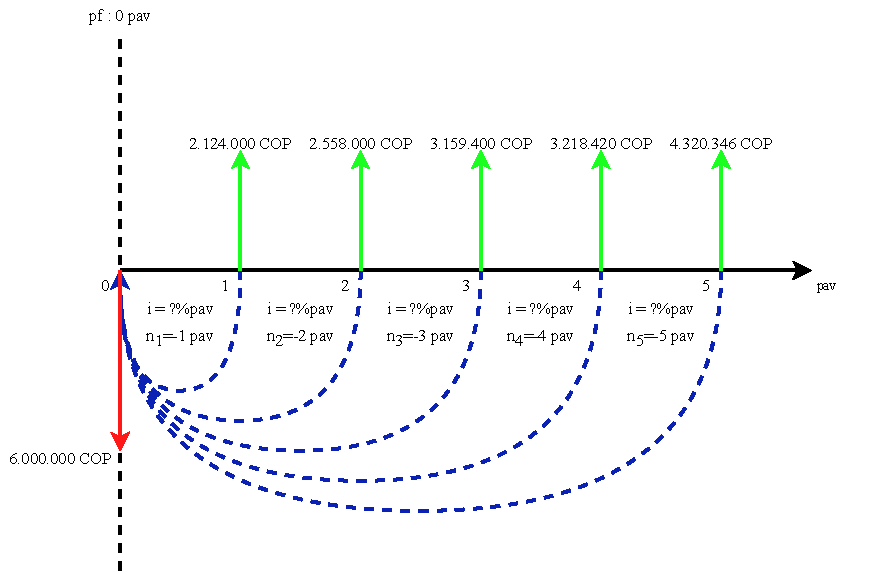
\includegraphics[scale=0.8]{ejemplos/7/Graf1Ej7Cap11.pdf} }
		\\ \hline
		%%%%%%%%%%%%% FIN INSERCIÓN DE IMAGEN
		%%%FIN DIAGRAMA DE FLUJO



		%%%%% INICIO DECLARACIÓN FORMULAS
		%%%%%%%%%%% INICIO TITULO
		\rowcolor[HTML]{FFB183}
		\multicolumn{3}{|c|}{\cellcolor[HTML]{FFB183}\textbf{4. Declaración de fórmulas}}                                                                                                                                                                                              \\ \hline
		%%%%%%%%%%% FIN TITULO
		%%%%%%%%%%% INICIO MATEMÁTICAS
		\multicolumn{3}{|c|} {$ \text{Base = Ingreso — Costo — Depreciación.} $}                                                                                                                                                                                                       \\
		\multicolumn{3}{|c|} {$ \text{Impuesto = Tasa impositiva x Base} $}                                                                                                                                                                                                            \\
		\multicolumn{3}{|c|} {$ \textbf{Flujo Neto de Caja: } \text{FNC = Ingreso — Costo — Impuesto } $}                                                                                                                                                                              \\
		\multicolumn{3}{|c|} {$VPN =\sum F_{n}(1+i)^{-n} $ Valor presente neto.}                                                                                                                                                                                                       \\
		\hline

		%%%%%%%%%% FIN MATEMÁTICAS
		%%%%%% INICIO DESARROLLO MATEMÁTICO
		\rowcolor[HTML]{FFB183}
		%%%%%%%%%%INICIO TITULO
		\multicolumn{3}{|c|}{\cellcolor[HTML]{FFB183}\textbf{5. Desarrollo matemático}}                                                                                                                                                                                                \\ \hline
		%%%%%%%%%% FIN TITULO
		%%%%%%%%%% INICIO MATEMÁTICAS
		\multicolumn{3}{|c|}{$ \text{A continuación presentamos la tabla necesaria para calcular el flujo de caja.} $}
		\\
		%%\multicolumn{3}{|c|}{ \includegraphics[scale=0.7]{7/Graf2Ej7Cap11.pdf} }   
		\multicolumn{3}{|c|}{ }
		\\
		\multicolumn{3}{|c|}{}                                                                                                                                                                                                                                                         \\
		\multicolumn{3}{|c|}{
			{\fontsize{8.5}{10}\selectfont
					\begin{tabular}{|>{\centering\arraybackslash}p{0.3cm}|>{\centering\arraybackslash}p{1.8cm}|>{\centering\arraybackslash}p{1.9cm}|>{\centering\arraybackslash}p{1.8cm}|>{\centering\arraybackslash}p{1.9cm}|>{\centering\arraybackslash}p{1.9cm}|>{\centering\arraybackslash}p{1.9cm}|}
						\hline
						\rowcolor{white!50}
						\textbf{Per} & \textbf{Ingreso}                   & \textbf{Costo}                     & \textbf{Depreciación}              & \textbf{Base}                      & \textbf{Impuesto}                  & \textbf{FNC}                       \\ \hline
						\text{0}     & \text{6\text{.}000\text{.}000 COP} & \text{0 COP}                       & \text{0 COP}                       & \text{0 COP}                       & \text{0 COP}                       & \text{6\text{.}000\text{.}000 COP} \\ \hline
						\text{1}     & \text{3\text{.}000\text{.}000 COP} & \text{800\text{.}000 COP}          & \text{2\text{.}000\text{.}000 COP} & \text{200\text{.}000 COP}          & \text{76\text{.}000 COP}           & \text{2\text{.}124\text{.}000 COP} \\ \hline
						\text{2}     & \text{3\text{.}900\text{.}000 COP} & \text{1\text{.}000\text{.}000 COP} & \text{2\text{.}000\text{.}000 COP} & \text{900\text{.}000 COP}          & \text{342\text{.}000 COP}          & \text{2\text{.}558\text{.}000 COP} \\ \hline
						\text{3}     & \text{5\text{.}070\text{.}000 COP} & \text{1\text{.}200\text{.}000 COP} & \text{2\text{.}000\text{.}000 COP} & \text{1\text{.}870\text{.}000 COP} & \text{710\text{.}000 COP}          & \text{3\text{.}159\text{.}400 COP} \\ \hline
						\text{4}     & \text{6\text{.}591\text{.}000 COP} & \text{1\text{.}400\text{.}000 COP} & \text{-}                           & \text{5\text{.}191\text{.}000 COP} & \text{1\text{.}972\text{.}000 COP} & \text{3\text{.}218\text{.}420 COP} \\ \hline
						\text{5}     & \text{8\text{.}568\text{.}300 COP} & \text{1\text{.}600\text{.}000 COP} & \text{-}                           & \text{6\text{.}968\text{.}000 COP} & \text{2\text{.}647\text{.}954 COP} & \text{4\text{.}320\text{.}346 COP} \\ \hline
					\end{tabular}
				}
		}                                                                                                                                                                                                                                                                              \\
		\multicolumn{3}{|c|}{ }                                                                                                                                                                                                                                                        \\
		\multicolumn{3}{|c|}{$ \text{Si hacemos el VPN = 0 podemos hallar la TIR.} $}
		\\
		\multicolumn{3}{|c|}{$VPN = -6\text{.}000\text{.}000 COP +  2\text{.}124\text{.}000 COP(1+i)^{-1} +  2\text{.}558\text{.}000 COP(1+i)^{-2} $}
		\\
		\multicolumn{3}{|c|}{$ +3\text{.}159\text{.}400 COP(1+i)^{-3} + 3\text{.}218\text{.}420 COP(1+i)^{-4} +  4\text{.}320\text{.}346 COP(1+i)^{-5} = 0 \text{ COP}$}
		\\
		\multicolumn{3}{|c|}{$ \text{Al resolver esta ecuación por interpolación se obtiene:} $}
		\\
		\multicolumn{3}{|c|}{$ \text{i = 36,58\% pav} $}
		\\
		\hline

		%%%%%%%%%% FIN MATEMÁTICAS
		%%%%%% FIN DESARROLLO MATEMÁTICO
		%%%%%% INICIO RESPUESTA
		\rowcolor[HTML]{FFB183}
		%%%%%%%%%%INICIO TITULO
		\multicolumn{3}{|c|}{\cellcolor[HTML]{FFB183}\textbf{6. Respuesta}}                                                                                                                                                                                                            \\ \hline
		%%%%%%%%%% FIN TITULO
		%%%%%%%%%% INICIO RESPUESTA MATEMÁTICA

		\multicolumn{3}{|c|}{ $\text{La rentabilidad del proyecto es del 36,58\% pav}$}
		\\
		\hline


		%%%%%%%%%% FIN MATEMÁTICAS
		%%%%%% FIN RESPUESTA
	\end{longtable}
	%Se crean dos lineas en blanco para que no quede el siguiente texto tan pegado
	%\newline \newline %USARLO SI CREES QUE ES NECESARIO
\end{center}
%%%%%%%%%%%%%%%%%%%%%%%%%%FIN EJERCICIO 1 %%%%%%%%%%%%%%%%%%%%%%%%%%%

